\documentclass[rusmathsym, eqnumwithinsec, amspack, hyperref]{bomgost}

\DeclareTextSymbol{\CYRA}\UnicodeEncodingName{"0410}        % А
\DeclareTextSymbol{\cyra}\UnicodeEncodingName{"0430}        % а
\DeclareTextSymbol{\CYRB}\UnicodeEncodingName{"0411}        % Б
\DeclareTextSymbol{\cyrb}\UnicodeEncodingName{"0431}        % б
\DeclareTextSymbol{\CYRV}\UnicodeEncodingName{"0412}        % В 
\DeclareTextSymbol{\cyrv}\UnicodeEncodingName{"0432}        % в
\DeclareTextSymbol{\CYRG}\UnicodeEncodingName{"0413}        % Г
\DeclareTextSymbol{\cyrg}\UnicodeEncodingName{"0433}        % г
\DeclareTextSymbol{\CYRD}\UnicodeEncodingName{"0414}        % Д
\DeclareTextSymbol{\cyrd}\UnicodeEncodingName{"0434}        % д
\DeclareTextSymbol{\CYRE}\UnicodeEncodingName{"0415}        % Е 
\DeclareTextSymbol{\cyre}\UnicodeEncodingName{"0435}        % е
\DeclareTextSymbol{\CYRZH}\UnicodeEncodingName{"0416}       % Ж 
\DeclareTextSymbol{\cyrzh}\UnicodeEncodingName{"0436}       % ж
\DeclareTextSymbol{\CYRZ}\UnicodeEncodingName{"0417}        % З
\DeclareTextSymbol{\cyrz}\UnicodeEncodingName{"0437}        % з
\DeclareTextSymbol{\CYRI}\UnicodeEncodingName{"0418}        % И
\DeclareTextSymbol{\cyri}\UnicodeEncodingName{"0438}        % и
\DeclareTextSymbol{\CYRISHRT}\UnicodeEncodingName{"0419}    % Й
\DeclareTextSymbol{\cyrishrt}\UnicodeEncodingName{"0439}    % й
\DeclareTextSymbol{\CYRK}\UnicodeEncodingName{"041A}        % К
\DeclareTextSymbol{\cyrk}\UnicodeEncodingName{"043A}        % к
\DeclareTextSymbol{\CYRL}\UnicodeEncodingName{"041B}        % Л
\DeclareTextSymbol{\cyrl}\UnicodeEncodingName{"043B}        % л 
\DeclareTextSymbol{\CYRM}\UnicodeEncodingName{"041C}        % М
\DeclareTextSymbol{\cyrm}\UnicodeEncodingName{"043C}        % м
\DeclareTextSymbol{\CYRN}\UnicodeEncodingName{"041D}        % Н
\DeclareTextSymbol{\cyrn}\UnicodeEncodingName{"043D}        % н
\DeclareTextSymbol{\CYRO}\UnicodeEncodingName{"041E}        % О
\DeclareTextSymbol{\cyro}\UnicodeEncodingName{"043E}        % о
\DeclareTextSymbol{\CYRP}\UnicodeEncodingName{"041F}        % П
\DeclareTextSymbol{\cyrp}\UnicodeEncodingName{"043F}        % п
\DeclareTextSymbol{\CYRR}\UnicodeEncodingName{"0420}        % Р
\DeclareTextSymbol{\cyrr}\UnicodeEncodingName{"0440}        % р
\DeclareTextSymbol{\CYRS}\UnicodeEncodingName{"0421}        % С
\DeclareTextSymbol{\cyrs}\UnicodeEncodingName{"0441}        % с
\DeclareTextSymbol{\CYRT}\UnicodeEncodingName{"0422}        % Т
\DeclareTextSymbol{\cyrt}\UnicodeEncodingName{"0442}        % т
\DeclareTextSymbol{\CYRU}\UnicodeEncodingName{"0423}        % У
\DeclareTextSymbol{\cyru}\UnicodeEncodingName{"0443}        % у
\DeclareTextSymbol{\CYRF}\UnicodeEncodingName{"0424}        % Ф
\DeclareTextSymbol{\cyrf}\UnicodeEncodingName{"0444}        % ф
\DeclareTextSymbol{\CYRH}\UnicodeEncodingName{"0425}        % Х
\DeclareTextSymbol{\cyrh}\UnicodeEncodingName{"0445}        % х
\DeclareTextSymbol{\CYRC}\UnicodeEncodingName{"0426}        % Ц
\DeclareTextSymbol{\cyrc}\UnicodeEncodingName{"0446}        % ц
\DeclareTextSymbol{\CYRCH}\UnicodeEncodingName{"0427}       % Ч
\DeclareTextSymbol{\cyrch}\UnicodeEncodingName{"0447}       % ч
\DeclareTextSymbol{\CYRSH}\UnicodeEncodingName{"0428}       % Ш
\DeclareTextSymbol{\cyrsh}\UnicodeEncodingName{"0448}       % ш
\DeclareTextSymbol{\CYRSHCH}\UnicodeEncodingName{"0429}     % Щ
\DeclareTextSymbol{\cyrshch}\UnicodeEncodingName{"0449}     % щ
\DeclareTextSymbol{\CYRHRDSN}\UnicodeEncodingName{"042A}    % Ъ
\DeclareTextSymbol{\cyrhrdsn}\UnicodeEncodingName{"044A}    % ъ
\DeclareTextSymbol{\CYRERY}\UnicodeEncodingName{"042B}      % Ы
\DeclareTextSymbol{\cyrery}\UnicodeEncodingName{"044B}      % ы
\DeclareTextSymbol{\CYRSFTSN}\UnicodeEncodingName{"042C}    % Ь
\DeclareTextSymbol{\cyrsftsn}\UnicodeEncodingName{"044C}    % ь
\DeclareTextSymbol{\CYREREV}\UnicodeEncodingName{"042D}     % Э
\DeclareTextSymbol{\cyrerev}\UnicodeEncodingName{"044D}     % э
\DeclareTextSymbol{\CYRYU}\UnicodeEncodingName{"042E}       % Ю
\DeclareTextSymbol{\cyryu}\UnicodeEncodingName{"044E}       % ю
\DeclareTextSymbol{\CYRYA}\UnicodeEncodingName{"042F}       % Я
\DeclareTextSymbol{\cyrya}\UnicodeEncodingName{"044F}       % я

% Закомментируйте это, если hyperref не нужен. 
% Изменение уровня \subparagraph (приложения) в закладках pdf документа. 
% Это нужно для сохранения правильной иерархии закладок в pdf документе.
\makeatletter%
\renewcommand{\toclevel@subparagraph}{2}%
\makeatother% 

% Для вставки программного кода.
\usepackage{listings}

% "Умная" запятая: \(0,2\) - число, \(0, 2\) - перечисление.
\usepackage{icomma}
\usepackage{float}
\usepackage{pgfplots}
\usepackage{pgfplotstable}
\usepackage{longtable}
\usepackage{cleveref}


\pgfplotsset{compat=newest}

\pgfplotstableset{set thousands separator={}, precision=3, use comma, col sep=comma, header=true,
every head row/.style={before row=\hline, after row=\hline},
every even row/.style={after row=\hline},
every odd row/.style={after row=\hline},
every column/.style={column type/.add={|}{}},
every last column/.style={column type/.add={}{|}},
columns/text/.style={string type},
}

\author{Кухта А.В.}
\title{Разработка устройства для калибровки для исследования характеристик антенно-фидерного и приёмного тракта иркутского радара}
\date{\today}


\begin{document}

\maketitle
\thispagestyle{empty}
\newpage

\begin{abstract}
% Для добавления общего числа приложений нужно добавить команду \printtotapp[.]
% Во всех командах существует необязательный аргумент, который добавляется в конец команды. По умолчанию это запятая. Это нужно для случаев, когда каких-то элементов в работе нет т. е. их счётчики равны 0. В этом случае команда ничего не выведет. Так как порядок команд может быть любым и необходимо, чтобы после последней команды была точка, а между командами запятая, поэтому добавлен необязательный аргумент.
Выпускная квалификационная работа содержит \printtotpage \printtotfig \printtottab \printtotref[.] В~некоторых случаях количество приложений не указывается. 

% Для количества приложений команда аналогична: \total{totappendix}~приложений.

КЛЮЧЕВОЕ СЛОВО~1, КЛЮЧЕВОЕ СЛОВО~2, КЛЮЧЕВОЕ СЛОВО~3 и т. д.

Краткое описание работы.
\end{abstract}


\tableofcontents


\section*{ОБОЗНАЧЕНИЯ И СОКРАЩЕНИЯ}
ОДУ - обыкновенные дифференциальные уравнения.

СЛАУ - система линейных алгебраических уравнений.

%
% ВВЕДЕНИЕ
%

\section*{ВВЕДЕНИЕ}
Используя отладочную плату NUCLEO-F746ZG на основе микроконтроллера STM32 и синтезатор на основе чипа AD9910, необходимо создать программное обеспечение (ПО) для микропроцессора и разработать генератор тестовых сигналов для калибровки и диагностики Иркутского радара некогерентного рассеяния (ИРНР).

ИРНР является уникальным инструментом. Всего в мире существует девять подобных радаров, а ИРНР — единственный в России. Он используется для изучения процессов, происходящих в ионосфере Земли, а также для экспериментов по наблюдению за космическими объектами.

Ниже представлены ключевые характеристики ИРНР из источника \cite{Kushnarev}:

\begin{itemize}
	\item Диапазон рабочих частот: 154–162 МГц.
	\item Пиковая мощность, достигаемая на двух передатчиках: 2.8 МВт.
	\item Длительность зондирующего импульса: от 70 до 900 мкс.
	\item Частота следования импульса: 24.4 Гц.
	\item Коэффициент усиления антенны: около 35 дБ.
\end{itemize}

ИРНР является радиолокационной станцией и во всех экспериментах крайне важно знать параметры всего приемо-передающего тракта, учитывать его задержки и нестабильность. Например, когда ИРНР работает в режиме наблюдения за космическими объектами, он использует задержку возвращения сигнала для определения расстояния до объекта. Для объектов на высоте 400 км, эта задержка составляет примерно 2600 мкс, и погрешность в одну микросекунду внесёт ~150 метров неточности в определённое расстояние. Следовательно, до проведения экспериментов необходимо измерить и учесть все задержки оборудования ИРНР и компенсировать их в дальнейшем.

Для решения этой задачи необходимо создать генератор тестовых сигналов. Он будет формировать сигналы с известными параметрами (длительность импульса, частота, задержка, уровень амплитуды, модуляция) и позволит измерить задержки оборудования, находящегося на пути следования сигнала.

Требования к генератору сигналов:

\begin{itemize}
	\item Возможность формирования сигналов на рабочих частотах ИРНР: 154–162 МГц.
	\item Длительность импульсов: от 100 до 1000 мкс.
	\item Заданная задержка для импульсов: от 150 до 10000 мкс.
	\item Возможность установки произвольных уровней амплитуды.
	\item Управление: по Ethernet или USB.
\end{itemize}

Выбор именно этих компонентов (отладочная плата Nucleo и синтезатор AD9910) был обусловлен уже имеющимися требованиями. Программная часть состоит из прошивки для микроконтроллера, написанной на языке программирования C. Для создания прошивки использовалась среда разработки VSCode и компилятор GCC.



\mainpart


\section{ТЕОРЕТИЧЕСКАЯ ЧАСТЬ}
\subsection{Цифровые синтезаторы частот}

Цифровые синтезаторы частот, также известные как DDS (Direct Digital Synthesizer), являются классом устройств, которые предназначены для создания сигнала с настраиваемой частотой, фазой и амплитудой.

DDS используются:

\begin{itemize}
	\item В качестве источников тактовой частоты в тех задачах, где требуется изменение тактовой частоты в реальном времени.
	\item В качестве модуляторов для передачи данных.
	\item В атомных интерферометрах.
	\item В радарах.
\end{itemize}

В отличие от SDR с возможностью передачи (напр. HackRF), DDS, как правило, не предназначены для получения сигналов полностью произвольной формы, но всё равно способны создать широкий набор сигналов.

Главными характеристиками DDS являются:

\begin{itemize}
	\item Разрядность аккумулятора фазы (напр. 24, 32 или 48 бит), от которой зависит точность выбора частоты сигнала.
	\item Максимальная внутренняя частота, от которой зависит максимальная синтезируемая частота.
\end{itemize}

Исчерпывающее описание принципов работы DDS можно найти в источнике \cite{DDSTutorial}.

\subsection{Формирование сигналов}

Использование калибратора предполагается в сочетании с некоторым записывающим устройством, подробности которого не рассматривается в рамках этой работы.

Задача калибратора состоит в том, чтобы создавать сигналы заранее известной формы, которые затем записываются записывающим устройством после прохождения через некоторую среду.

Прохождение сигнала через среду может исказить его–под искажением понимается любое изменение сигнала–и это искажение требуется характеризовать.

Искажения можно выразить через амплитудно-частотную характеристику (АЧХ) и фазово-частотную характеристику (ФЧХ).

Амплитудно-частотная характеристика описывает уровень амплитуды в зависимости от частоты после прохождения через среду и отражает затухание разных частот.

\subsection{Спектральный анализ}

Имея запись некоторого сигнала, можно найти количество некоторой частотной составляющей в нём, вычислив сумму произведений этого сигнала и сигнала, полностью заполненного сигналом интересующей частоты. Это работает, так как:

% https://tex.stackexchange.com/questions/47170/how-to-write-conditional-equations-with-one-sided-curly-brackets
\begin{equation}
	\int_{-\infty}^{\infty}{\sin(ax)\sin(bx)}{dx}
	\begin{cases}
		\infty,& a = b\\
		0,     & a \neq b
	\end{cases}
\end{equation}

Можно проверить, что это действительно так, при помощи небольшой программы на Python с использованием библиотеки numpy, которая вычисляет сумму произведений двух сигналов, для случая с сигналами одинаковой частоты и разной частоты:

% https://tex.stackexchange.com/questions/106770/how-to-add-line-numbers-to-a-program-listing-code
\lstset{
	language=python,
	basicstyle=\ttfamily,
    numbers=left,
    stepnumber=1,
    showstringspaces=false,
    tabsize=4,
    breaklines=true,
    breakatwhitespace=false,
}
\begin{lstlisting}
import numpy as np

x = np.arange(1000)

print( np.sin(x) @ np.sin(x) )   # 499.5
print( np.sin(x) @ np.sin(2*x) ) # -0.01
\end{lstlisting}

В приведённом выше примере рассматривается случай с извлечением составляющих с известной частотой и известной начальной фазой, то есть сигналы вида $\sin(x+0)$. Если же начальная фаза не известна, как часто бывает на практике, то её можно извлечь исходя из следующего:

\begin{equation}
	\int_{-\infty}^{\infty}{\sin(x)\cos(x)}{dx}=0
\end{equation}

А также формулы суммы тригонометрических функций, когда, например, $\sin(x+2)$ на самом деле является $\cos(2)\sin(x) + \sin(2)\cos(x)$, или примерно $-0.416\sin(x) + 0.909\cos(x)$

\subsubsection{Рисунок}
График представлен на рисунке ниже.
% Важно добавлять каждый рисунок в окружение gostfigure, чтобы был правильный подсчёт общего числа рисунков.
\begin{gostfigure}
\begin{figure}[H]
\centering
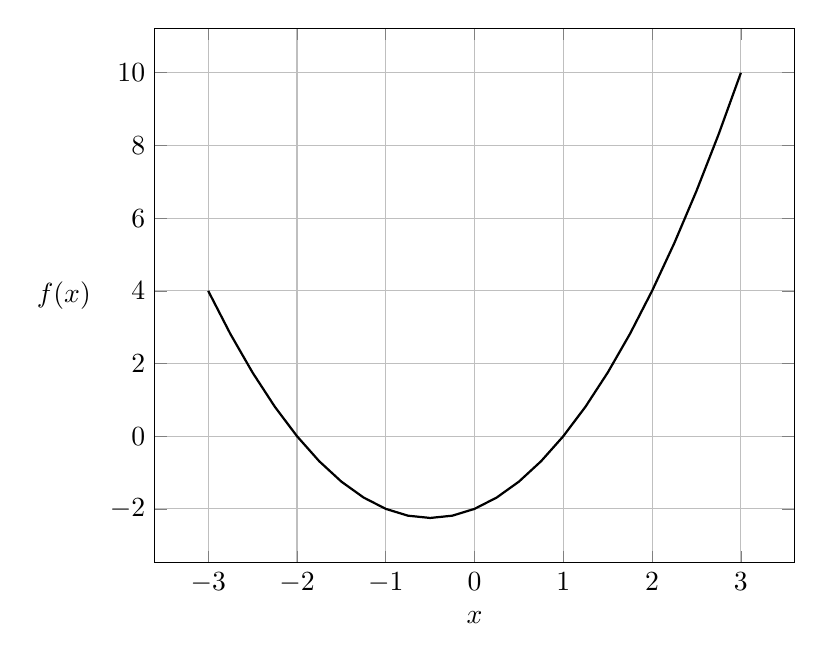
\begin{tikzpicture}
  \begin{axis}[domain=-3:3, width = 0.8 \textwidth, grid = both, ylabel style={rotate=-90}, xlabel = \(x\), ylabel = \(f(x)\)]
  \addplot[mark=none, thick]{x*x + x - 2};
  \end{axis}
\end{tikzpicture}
\caption{График \(f(x)\).}
\end{figure}
\end{gostfigure}

Корни квадратного уравнения представлены в~таблице~\ref{tab:roots}.
% Аналогично с таблицами.
\begin{gosttable}
\begin{table}[H]
\centering
\caption{Корни квадратного уравнения.}
\label{tab:roots}
\begin{tabular}{|c|c|}
\hline 
Первый корень &  Второй корень \\ 
\hline 
1 & -2  \\ 
\hline 
\end{tabular}
\end{table}
\end{gosttable}

\subsection{Таблица из файла}

Пример таблицы из файла, которую просто обновлять.

\pgfplotstableread{data/sample.csv}{\loadedtable}

\begin{gosttable}
    \begin{table}[H]
        \centering
        \caption{Табличные данные}
        \pgfplotstabletypeset[columns={id,num}]{\loadedtable}
    \end{table}
\end{gosttable}

Другие столбцы.

\begin{gosttable}
  \begin{table}[H]
      \centering
      \caption{Табличные данные}
      \pgfplotstabletypeset[columns={id,text}]{\loadedtable}
  \end{table}
\end{gosttable}

\subsubsection{Таблица с разрывом страницы}
\pgfplotstableread{data/big.csv}{\loadedtable}
\begin{gosttable}
  \pgfplotstabletypeset[font=\small
  ,begin table = \begin{longtable}
  ,end table = \end{longtable}
  ,every head row/.append style={before  row={%
  \caption{Таблица с разрывом}
  \label{tab:long_table}\\
  \hline
  \endfirsthead
  \caption*{Продолжение таблицы~\cref{tab:long_table}}\\
  \hline 
  col 1 & col 2 & col 3\\
  \hline
  \endhead
  }
  }
  ,every first row/.append style={before row ={
    col 1 & col 2 & col 3\\
  \hline
  }
  }
  , columns={id,num,text}
  ]{\loadedtable}
\end{gosttable}

%
% Практическая часть
%
\section{ПРАКТИЧЕСКАЯ ЧАСТЬ}
\subsection{Описание устройства}

Устройство представляет из себя генератор сигналов, предназначенный для подачи коротких сигналов (импульсов) по внешнему событию (триггеру) с возможностью настройки параметров сигналов и задания последовательностей сигналов с разными параметрами.

В состав устройства входят: отладочная плата AD9910 PCBZ с синтезатором и отладочная плата Nucleo F746ZG с микроконтроллером, а также мезонинная плата, которая выводит необходимые управляющие сигналы с микроконтроллера и предоставляет необходимые напряжения питания.

Ниже представлено схематическое изображение устройства:

%
% Блок-схема устройства
%
\begin{gostfigure}
\begin{figure}[H]
\centering
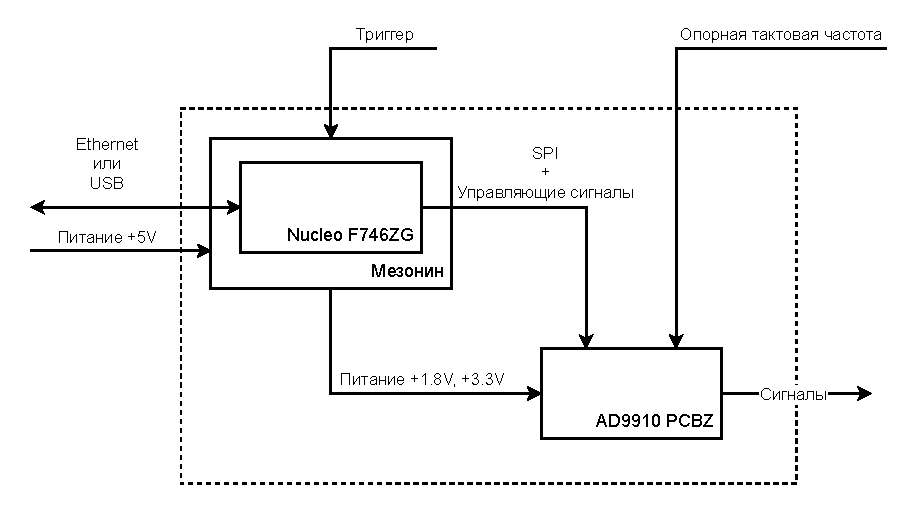
\includegraphics{data/system_architecture.drawio.pdf}
\caption{Общая схема устройства.}
\label{fig:system_architecture}
\end{figure}
\end{gostfigure}

Управление устройством осуществляется c ПК по USB или Ethernet, через виртуальный ком-порт в первом случае и через утилиту netcat во втором случае. Устройство предоставляет текстовый интерфейс, который включает в себя комманды добавления сигналов в очередь, очистки очереди, запуска и остановки воспроизведения из очереди.

\pagebreak

Триггер может предоставлятся как внешним устройством, так и самим микроконтроллером: на мезонинной плате предусмотрена перемычка, которая позволяет выбирать внешний либо внутренний источник. Частота следования триггеров может варьироваться в разумных пределах; внутренний источник сконфигурирован под стробирующий сигнал с частотой 25 Гц.

Ниже представлено схематичное изображение процесса подачи сигналов, схожее с тем, что можно было бы увидеть на осциллоскопе:

%
% Схематичное изображение процесса работы
%
\begin{gostfigure}
\begin{figure}[H]
\centering
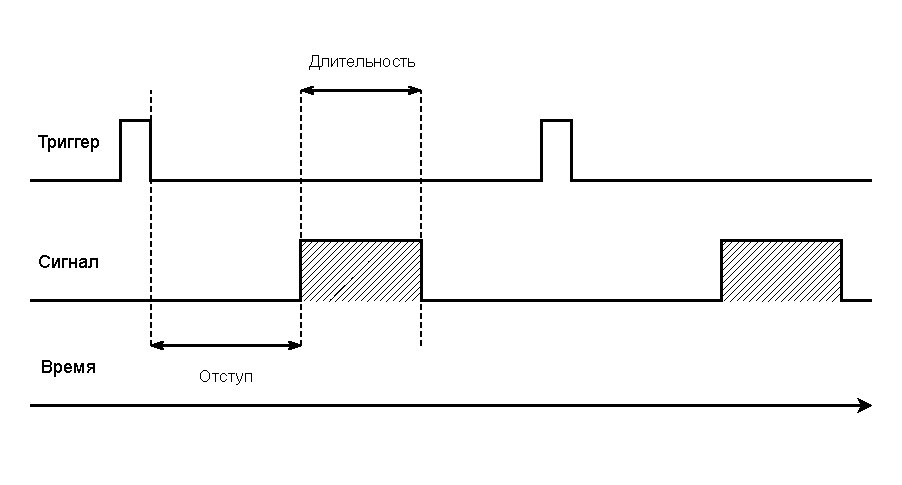
\includegraphics{data/timing_diagram.drawio.pdf}
\caption{Подача сигналов.}
\label{fig:timing_diagram}
\end{figure}
\end{gostfigure}

\subsection{Программирование}

Прошивка для микроконтроллера написана на языке программирования C, с использованием преимущественно свободных инструментов с открытым исходным кодом.

В качестве компилятора C использован gcc для ARM; все используемые в проекте библиотеки нацелены именно на этот компилятор, что и послужило главной причиной для его выбора. Возможной альтернативой является компилятор clang в составе проекта LLVM, но не проверялось, сможет ли он без ошибок собрать все задействованные библиотеки, в особенности STM32 HAL, который может содержать специфичный для gcc код.

В качестве системы сборки использован GNU Make. Задача Make состоит в запуске команд сборки, также называемых правилами, для каждого файла с исходным кодом. Главное преимущество от использования Make по сравнению с, например, скриптом сборки для интерпретатора командной строки, будь это bash или что-нибудь другое, заключается в возможности параллельной сборки, когда не зависящие друг от друга файлы с исходным кодом собираются параллельно, что позволяет существенно ускорить полную сборку проекта. Другим преимуществом является поддержка частичной сборки, когда повторно компилируются только файлы, изменившиеся с момента предыдущей сборки. Нужно отметить, что существуют и другие системы сборки, например CMake и ninja, которые обладают схожими возможностями, но часто сложнее в использовании.

В качестве IDE использована среда разработки VSCode, которая была выбрана преимущественно в связи с её популярностью и наличием расширения C/C++ IntelliSense, которое предоставляет быстрый поиск идентификаторов во всех файлах проекта и является незаменимым инструментом при изучении кода больших библиотек, таких как STM32 HAL. Нужно отметить, что, в отличие от самого VSCode, это расширение не является полностью свободным — его исходный код закрыт. Другими IDE, которе бы подошли для разработки прошивки под ARM устройство, являются Qt Creator и CLion.

В качестве инструмента для загрузки собранной прошивки в микроконтроллер а также отладки использован OpenOCD. Этот инструмент позволяет прошивать множество микроконтроллеров от разных производителей а также выступает сервером отладки для gdb.

Наконец, в качестве отладчика использован gdb, который не имеет возможности самостоятельно взаимодействовать с отлаживаемым устройством и полагается на OpenOCD в качестве сервера.

\subsection{Использование AD9910}

Цифровой синтезатор сигналов (DDS) AD9910 представлен в исполнении производителя на отладочной плате AD9910 PCBZ. Данная плата предусматривает управление при помощи внешнего микроконтроллера, либо с ПК при помощи интерфейса USB, который реализован неизвестным микроконтроллером на плате.

В режиме управления с ПК, синтезатор подключается по USB, и используя утилиту от производителя (представлена на рисунке \ref{fig:ad9910_evaluation_software}) можно управлять всеми его настройками, видя при этом изменения в содержимом регистров. Это крайне полезный инструмент для ознакомления с устройством.

\begin{gostfigure}
\begin{figure}[H]
\centering
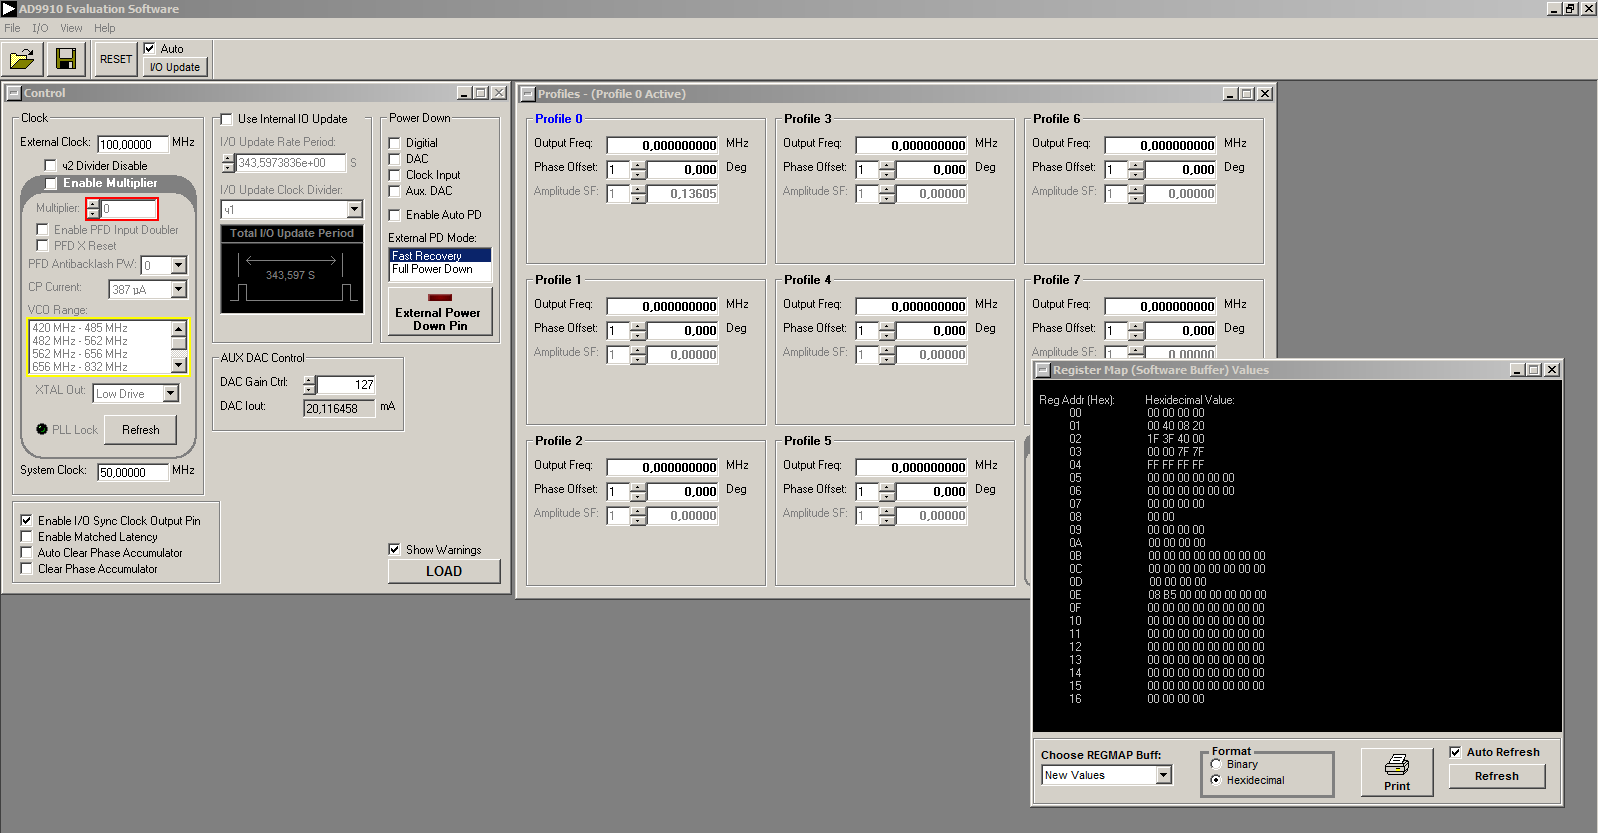
\includegraphics[scale=.25]{data/ad9910_evaluation_software.png}
\caption{Утилита управления синтезатором AD9910 с ПК.}
\label{fig:ad9910_evaluation_software}
\end{figure}
\end{gostfigure}

Всего синтезатор имеет 23 регистра с различной шириной, от 2 байт до 8 байт. В большинстве случаев, один бит регистра отвечает за включение/выключение некоторой функции синтезатора, но есть некоторые регистры, которые отведены под хранение числовых значений, например регистры 15-22 используются для хранения восьми профилей генерируемой частоты. Полное описание полей регистров чипа AD9910 можно найти в источнике [6].

Расположенный на плате синтезатора микроконтроллер не подходит для решения поставленной задачи по двум причинам: во-первых, у него нет интерфейса Ethernet, а это является одним из требований к устройству. Во-вторых, исходные коды его существующей прошивки нигде не доступны. Поэтому встроенный микроконтроллер был отключен перестановкой перемычек на плате.

Управление внешним микроконтроллером осуществляется при помощи множества выделенных под отдельные функции синтезатора управляющих сигналов а также SPI для доступа к регистрам.

По умолчанию, синтезатор запускается в двухпроводном режиме SPI, когда задействованы только линии MOSI и SCK устройства-мастера. Запись данных происходит в обычном для SPI режиме, а для чтения MOSI временно переключается в режим входа на устройстве-мастере. Чтобы включить трёхпроводной режим, необходимо обновить значение в регистре CFGR0.

В рамках одной транзакции данных синтезатору сначала отправляется инструкция размером в один байт, где старший бит выбирает между режимом записи и режимом чтения, а пять младших битов определяют номер интересующего регистра. В режиме записи должны последовать {\em n} байт, где {\em n} — ширина регистра, а в режиме чтения, наоборот, должно быть считано {\em n} байт.

Используемые для SPI входы и выходы представлены в таблице \ref{tab:spi_pins}:

% %%%%%%%%%%%%%%%%%%%%%%%%%%%%%%%%%%%%%%%%%%%%%%%%%%%%
% Таблица используемых для SPI входов и выходов AD9910
% %%%%%%%%%%%%%%%%%%%%%%%%%%%%%%%%%%%%%%%%%%%%%%%%%%%%
\begin{table}[H]
\centering
\caption{Используемые для SPI входы и выходы AD9910}
\label{tab:spi_pins}
\begin{tabular}{|p{4cm}|p{8cm}|}
\hline 
\textbf{Название} & \textbf{Пояснение} \\ 
\hline 
CSB & Низкий уровень на этом входе активирует порт SPI синтезатора \\ 
\hline
SCLK & Тактовый сигнал SPI подаваемый устройством-мастером \\
\hline
SDO & Выход SPI для отправки данных устройству-мастеру \\
\hline
SDIO & Вход SPI для получения данных от устройства-мастера, или вход и выход одновременно, в зависимости от выбранного режима SPI \\
\hline 
IO\_RESET & Высокий уровень на этом входе отменяет текущую транзакцию \\
\hline
\end{tabular} 
\end{table}

Одна из первых проблем, с которыми мы столкнулись, заключалась в том, что синтезатор никак не реагировал на команды по SPI:

\section*{ЗАКЛЮЧЕНИЕ}
Интересная стать~\cite{Cybenko}, связанная с~нейронными сетями.

% Список литературы.
\begin{thebibliography}{11}
\bibitem{DDSTutorial} A Technical Tutorial
on Digital Signal Synthesis https://www.ieee.li/pdf/essay/dds.pdf
\bibitem{Kushnarev} Кушнарев Д.С., Лебедев В.П., Хахинов В.В., Евстифеев С.Е., Заруднев В.Е. Модернизация Иркутского радара некогерентного рассеяния. Солнечно-земная физика. 2017. Т. 3, № 3. С. 88-94.
\bibitem{Volterra} Вольтерра В. Математическая теория борьбы за существование // Усп. физ. наук. 1928. № 1 (8). C. 13–34.
\bibitem{Cybenko} Cybenko G. Approximation by Superpositions of a Sigmoidal Function // Mathematics of Control, Signals, and Systems. 1989. (2). C. 303–314.
\end{thebibliography}

\appendix

\begin{gostappendix}{Программный код}
\lstset{language=[11]c++,basicstyle=\ttfamily, showstringspaces=false}

\begin{lstlisting}
#include <iostream>

using namespace std;

int main()
{
  auto b = 1;
  auto a = 2;
  cout << "2 + 1 = " << a + b << endl;
  return 0;
}
\end{lstlisting}
\end{gostappendix}


\begin{gostappendix}{Таблица}
aaa
\end{gostappendix}


\end{document}
